% fig-running-example.tex -- the running example of the introduction.
% Requires \usepackage{tikz} in the preamble (no extra TikZ library).
% Uses the paper macros \btrans and \Tr from main.tex.
% Geometry (all lengths in mm, exact up to pgfmath rounding):
%  (a) heights: one doubling of the density weight per 6.5mm step;
%  (b),(c) bar width = K*sqrt(weight), with one constant K for both panels;
%      (b) weight (3/4)16^{-m}: bar = 43/4^m, bars tile each row;
%      (c) weight (7/8)32^{-m}: bar = 43*sqrt(7/6)/sqrt(32)^m, centred in
%          the slot of width 43*sqrt(7/6)/4^m, so row m covers 2^{-m/2}.
\colorlet{rxaccent}{orange!80!black}%
\begin{tikzpicture}[x=1mm,y=1mm,font=\footnotesize,
  rxbar/.style={fill=black!10,draw=black!80,line width=0.25pt},
  rxhi/.style={fill=rxaccent!45,draw=rxaccent,line width=0.6pt},
  rxedge/.style={draw=black!55,line width=0.25pt},
  rxgrid/.style={draw=black!15,line width=0.3pt},
  rxarrow/.style={-stealth,line width=0.55pt,shorten <=0.9mm,shorten >=0.9mm}]
%
% ======================= (a) four doublings ==========================
% columns e_0..e_4 at x=12+7g; weight 2^{-j} (relative to xi) at y=-2.25-6.5j
\node[anchor=base west] at (3,7) {(a) one step down the tree};
\node[rotate=90,font=\scriptsize] at (48.6,-15.25) {weight, relative to $\xi$};
\foreach \g in {0,...,4}{
  \draw[rxgrid] ({12+7*\g},-0.6) -- ({12+7*\g},-29.9);
  \node[anchor=north] at ({12+7*\g},-30.6) {$e_{\g}$};
}
\foreach \rxj/\lab in {0/1,1/\frac12,2/\frac14,3/\frac18,4/\frac1{16}}{
  \draw[rxgrid] (10.4,{-2.25-6.5*\rxj}) -- (41.6,{-2.25-6.5*\rxj});
  \node[anchor=west,font=\scriptsize] at (42.6,{-2.25-6.5*\rxj}) {$\lab$};
}
% the four bridges: U_g carries e_{g-1} onto e_g and doubles the weight
\foreach \g in {1,...,4}{
  \draw[rxarrow] ({12+7*(\g-1)},{-2.25-6.5*(5-\g)}) -- ({12+7*\g},{-2.25-6.5*(4-\g)});
  \node[inner sep=0pt] at ({12+7*\g-3.5+1.75},{-2.25-6.5*(4-\g)-3.25-1.9}) {$\btrans_{\g}$};
}
% a_alpha: centralizer, weight unchanged
\draw[rxarrow] (12,-2.25) -- (40,-2.25);
\node[anchor=south] at (26,-2.0) {$a_\alpha$};
% A_alpha = v^* a_alpha on the root corner e_0: weight times 1/16
\draw[rxarrow,draw=rxaccent,line width=0.9pt] (12,-2.25) -- (12,-28.25);
\node[anchor=east,text=rxaccent] at (11.2,-15.25) {$A_\alpha$};
% points
\foreach \g in {1,...,3}{ \fill ({12+7*\g},{-2.25-6.5*(4-\g)}) circle (0.5); }
\fill (40,-2.25) circle (0.55);
\filldraw[fill=rxaccent,draw=rxaccent] (12,-2.25) circle (0.65);
\filldraw[fill=rxaccent,draw=rxaccent] (12,-28.25) circle (0.65);
\node[anchor=east] at (11.1,-2.25) {$\xi$};
\node[anchor=south] at (40,-1.3) {$a_\alpha\xi$};
\node[anchor=east] at (11.1,-28.25) {$A_\alpha\xi$};
%
% ======================= (b) four bridges ===========================
% x from 53 to 96 (width 43); row m occupies y in [-8m-4.5,-8m]
\node[anchor=base west] at (53,7) {(b) four bridges};
\node[anchor=base west,font=\scriptsize] at (53,2.2) {weight $\tfrac34\,16^{-m}$ per word};
\foreach \m in {1,2,3}{
  \pgfmathtruncatemacro{\rxN}{4^\m-1}
  \pgfmathsetmacro{\rxsc}{43/4^\m}
  \pgfmathsetmacro{\rxsp}{43/4^(\m-1)}
  \foreach \rxk in {0,...,\rxN}{
    \pgfmathtruncatemacro{\rxp}{floor(\rxk/4)}
    \draw[rxedge] ({53+(\rxp+0.5)*\rxsp},{-8*(\m-1)-4.5}) -- ({53+(\rxk+0.5)*\rxsc},{-8*\m});
  }
}
% each row is tiled exactly: one outline per row, each divider drawn once
\foreach \m in {0,...,3}{
  \draw[rxbar] (53,{-8*\m}) rectangle (96,{-8*\m-4.5});
}
\foreach \m in {1,2,3}{
  \pgfmathtruncatemacro{\rxN}{4^\m-1}
  \pgfmathsetmacro{\rxsc}{43/4^\m}
  \foreach \rxk in {1,...,\rxN}{
    \draw[draw=black!80,line width=0.25pt] ({53+\rxk*\rxsc},{-8*\m}) -- ({53+\rxk*\rxsc},{-8*\m-4.5});
  }
}
\draw[rxhi] (53,0) rectangle (96,-4.5);
\draw[rxhi] (63.75,-8) rectangle (74.5,-12.5);
\node[font=\scriptsize] at (74.5,-2.25) {$\emptyset$};
\foreach \rxk/\w in {0/00,1/01,2/10,3/11}{
  \node[font=\scriptsize] at ({53+(\rxk+0.5)*10.75},-10.25) {$\w$};
}
\node at (74.5,-31.2) {$\vdots$};
\node[anchor=base] at (74.5,-37.5) {$\Tr\sqrt{h_{F,1/16}}=\infty$};
%
% ======================= depth labels ===============================
\node[anchor=base,font=\scriptsize] at (100.5,2.2) {$m$};
\foreach \m in {0,...,3}{
  \node[font=\scriptsize] at (100.5,{-8*\m-2.25}) {$\m$};
}
%
% ======================= (c) five bridges ===========================
% same scale: root width 43*sqrt(7/6); x from 105
\pgfmathsetmacro{\rxW}{43*sqrt(7/6)}
\node[anchor=base west] at (105,7) {(c) five bridges};
\node[anchor=base west,font=\scriptsize] at (105,2.2) {weight $\tfrac78\,32^{-m}$ per word};
\foreach \m in {1,2,3}{
  \pgfmathtruncatemacro{\rxN}{4^\m-1}
  \pgfmathsetmacro{\rxsc}{\rxW/4^\m}
  \pgfmathsetmacro{\rxsp}{\rxW/4^(\m-1)}
  \foreach \rxk in {0,...,\rxN}{
    \pgfmathtruncatemacro{\rxp}{floor(\rxk/4)}
    \draw[rxedge] ({105+(\rxp+0.5)*\rxsp},{-8*(\m-1)-4.5}) -- ({105+(\rxk+0.5)*\rxsc},{-8*\m});
  }
}
\foreach \m in {0,...,3}{
  \pgfmathtruncatemacro{\rxN}{4^\m-1}
  \pgfmathsetmacro{\rxsc}{\rxW/4^\m}
  \pgfmathsetmacro{\rxbw}{\rxW/(sqrt(32)^\m)}
  \foreach \rxk in {0,...,\rxN}{
    \draw[rxbar] ({105+(\rxk+0.5)*\rxsc-0.5*\rxbw},{-8*\m}) rectangle ({105+(\rxk+0.5)*\rxsc+0.5*\rxbw},{-8*\m-4.5});
  }
}
\pgfmathsetmacro{\rxbwone}{\rxW/sqrt(32)}
\draw[rxhi] (105,0) rectangle ({105+\rxW},-4.5);
\draw[rxhi] ({105+1.5*\rxW/4-0.5*\rxbwone},-8) rectangle ({105+1.5*\rxW/4+0.5*\rxbwone},-12.5);
\node[font=\scriptsize] at ({105+0.5*\rxW},-2.25) {$\emptyset$};
\foreach \rxk/\w in {0/00,1/01,2/10,3/11}{
  \node[font=\scriptsize] at ({105+(\rxk+0.5)*\rxW/4},-10.25) {$\w$};
}
\node at ({105+0.5*\rxW},-31.2) {$\vdots$};
\node[anchor=base] at ({105+0.5*\rxW},-37.5) {$\Tr\sqrt{h_{F,1/32}}<\infty$};
\end{tikzpicture}%
